%%%%%%%%%%%%%%%%%%%%%%%%%%%%%%%%%%%%%%%%%%%%%%%%
% E.Pinault-Bigeard - e.pinault-bigeard@upsti.fr
% http://s2i.pinault-bigeard.com
% CC BY-NC-SA 2.0 FR - http://creativecommons.org/licenses/by-nc-sa/2.0/fr/
%%%%%%%%%%%%%%%%%%%%%%%%%%%%%%%%%%%%%%%%%%%%%%%%
\documentclass[11pt]{article}
%%%%%%%%%%%%%%%%%%%%%%%%%%%%%%%%%%%%%%%%%%%%%%%%
% Package UPSTI_Document
%%%%%%%%%%%%%%%%%%%%%%%%%%%%%%%%%%%%%%%%%%%%%%%%

\usepackage{import}
%
%%%%%%%%%%%%%%%%%%%%%%%%%%%%%%%%%%%%%%%%%%%%%%%%
% Package UPSTI_Document
%%%%%%%%%%%%%%%%%%%%%%%%%%%%%%%%%%%%%%%%%%%%%%%%
\usepackage{subcaption}
\usepackage[usenames, svgnames, dvipsnames]{xcolor}
\usepackage{UPSTI_Document}
\usepackage{pgfplots}
\usepackage{import}
\definecolor{darkspringgreen}{rgb}{0.09, 0.45, 0.27}

\newcommandx*{\dessinRepereFigGeo}[5][1=\vx{},2=\vy{},3=\vz{},4=,5=0]
	{
		\draw [->,very thick] (0,0) -- (1,0) ;
		\draw [->,very thick] (0,0) -- (0,1) ;
    \fill[white] (0,0) circle (0.13);
    \draw [->,very thick] (0,0) circle (0.13);
    \ifnumequal{#5}{0} {% z vers nous
      \fill[black] (0,0) circle (0.03);
      \draw [->,thick] (0,0) circle (0.04);
    }{% z vers la feuille
  		\begin{scope} [rotate=45]
  			\draw [-,thick] (0,-0.12) -- (0,0.12) ;
  			\draw [-,thick] (-0.12,0) -- (0.12,0) ;
  		\end{scope}
    }
		\draw [anchor=north west] (1.1,0) node {${#1}$};
		\draw [anchor=south west] (0,1.1) node {${#2}$};
		\draw [anchor=north east] (-0.1,0) node {${#3}$};
		\draw [anchor=north west] (-0.1,-0.1) node {${#4}$};
	}

	\usepackage{array}
	\newcolumntype{L}[1]{>{\raggedright\let\newline\\\arraybackslash\hspace{0pt}}m{#1}}
	\newcolumntype{C}[1]{>{\centering\let\newline\\\arraybackslash\hspace{0pt}}m{#1}}
	\newcolumntype{R}[1]{>{\raggedleft\let\newline\\\arraybackslash\hspace{0pt}}m{#1}}

	\usepackage{pifont}% http://ctan.org/pkg/pifont
\newcommand{\cmark}{\color{green}\ding{51}}%
\newcommand{\xmark}{\color{red}\ding{55}}%
\newcommand{\fmark}{\ding{229}}%
\newcommand{\itemc}{\item[\cmark]}%
\newcommand{\itemx}{\item[\xmark]}%
\newcommand{\itemf}{\item[\fmark]}%

\usepackage{csvsimple}
\usepackage{tikz-timing}
\usepackage{circuitikz}
\usepackage{pdfpages}
%---------------------------------%
% Paramètres du package
%---------------------------------%

% Version du document (pour la compilation)
% 1: Document prof
% 2: Document élève
% 3: Document à publier
\newcommand{\UPSTIidVersionDocument}{2}

% Classe
% 1: PTSI				6: PSI*			11: TSI2		16: Spé
% 2: PT	(par défaut)	7: MPSI			12: ATS
% 3: PT*				8: MP			13: PC
% 4: PCSI				9: MP*			14: PC*
% 5: PSI				10: TSI1		15: Sup
%\newcommand{\UPSTIidClasse}{2}



% Matière
% 1: S2I (par défaut)    2: IPT     3: TIPE
% 6: Vie au lycée
\newcommand{\UPSTIvariante}{5}
\newcommand{\UPSTIidMatiere}{0}
\newcommand{\UPSTIintituleMatiere}{Automatique}
\newcommand{\UPSTIsigleMatiere}{Autom}
% Type de document
% 0: Custom*				7: Fiche Métho de			14: Document Réponses
% 1: Cours (par défaut)		8: Fiche Synthèse    		15: Programme de colle
% 2: TD     				9: Formulaire
% 3: TP						10: Memo
% 4: Colle					11: Dossier Technique
% 5: DS						12: Dossier Ressource
% 6: DM						13: Concours Blanc
% * Si on met la valeur 0, il faut décommenter la ligne suivante:
%\newcommand{\UPSTItypeDocument}{Custom}
\newcommand{\UPSTIidTypeDocument}{1}

% Titre dans l'en-tête


% Titre dans l'en-tête

\newcommand{\UPSTIvariante}{5}

\newcommand{\UPSTItitreEnTete}{Automatisme industriel}
%\newcommand{\UPSTItitreEnTetePages}{}
\newcommand{\UPSTIsousTitreEnTete}{Introduction aux API}


% Titre
%\newcommand{\UPSTItitrePreambule}{Automatisme industriel}
\newcommand{\UPSTItitre}{La programmation d'un Automate Industriel}

% Durée de l'activité (pour DS, DM et TP)
\newcommand{\UPSTIduree}{3h30}

% Note de bas de première page
%\newcommand{\UPSTInoteBasDePremierePage}{Geoffrey Vaquette}
% Numéro (ajoute " n°1" après DS ou DM)
\newcommand{\UPSTInumero}{2}

% Numéro chapitre
%\newcommand{\UPSTInumeroChapitre}{1}

% En-tête customisé
%\newcommand{\UPSTIenTetePrincipalCustom}{UPSTIenTetePrincipalCustom}

% Message sous le titre
%\newcommand{\UPSTImessage}{Message sous le titre}


% Référence au programme
%\newcommand{\UPSTIprogramme}{\EPBComp \EPBCompP{B1-02}, \EPBCompP{B2-49}, \EPBCompS{B2-50}, \EPBCompS{B2-51}, \EPBCompP{C1-07}, \EPBCompP{C1-08}}

% Si l'auteur n'est pas l'auteur par défaut
%\renewcommand{\UPSTIauteur}{WWOOOOOOWW}

% Si le document est réalisé au nom de l'équipe
%\newcommand{\UPSTIdocumentCollegial}{1}

% Source
\newcommand{\UPSTIsource}{G. Vaquette}

% Version du document
\newcommand{\UPSTInumeroVersion}{1.0}

%-----------------------------------------------
\UPSTIcompileVars		% "Compile" les variables
%%%%%%%%%%%%%%%%%%%%%%%%%%%%%%%%%%%%%%%%%%%%%%%%


% Titre
%\newcommand{\UPSTItitrePreambule}{Automatisme industriel}
\newcommand{\UPSTItitre}{TP Test} 
\usetikzlibrary{arrows,automata,circuits.plc.ladder}

\newlength{\ladderskip}
\setlength{\ladderskip}{5\tikzcircuitssizeunit} % 5\tikzcircuitssizeunit = 35pt
\newlength{\ladderrungsep}
\setlength{\ladderrungsep}{.2\ladderskip}
\def\ladderrungend#1{\pgftransformyshift{-#1\ladderskip-\ladderrungsep}}

\ctikzset{
	logic ports=ieee,
	logic ports/scale=0.7,
}



\newcommand{\automaintienMachineEtat}[0]{
\begin{tikzpicture}[->,>=stealth',shorten >=1pt,auto,node distance=3cm,
                    semithick]
  %\tikzstyle{every state}=[fill=none,draw=none,text=white]

  \node[initial,state] (A)              {M1};
  \node[state]         (B) [right of=A] {M2};

  \path (A) edge [bend left]  node {$B_pM$} (B)
        (B) edge [bend left]  node {$B_pA$} (A);
\end{tikzpicture}
}


\newcommand{\sujet}{
	\exemplaire{1}{
	% En-tête
	\UPSTIbuildPage
	% \UPSTIamcZoneIdentification
	\begin{center}
			\noindent{}\fbox{\vspace*{3mm}
			\champnom{\Huge\bf\nom{}~\prenom{}~\id}\normalsize{}%
			\vspace*{3mm}
			\AMCassociation{\id}
		}
	\end{center}
	}

	

	\UPSTIboiteGenerique{Evaluation}{\bcplume}{Chaque activité sera implémentée sur un programme différent. N'attendez pas qu'un enseignant ait validé l'activité précédente avant de commencer le programme de la suivante.}
	\restituegroupe{combinatoire}
	\restituegroupe{sequentiel}
	\restituegroupe{analogique}
	\restituegroupe{machineAEtat}

	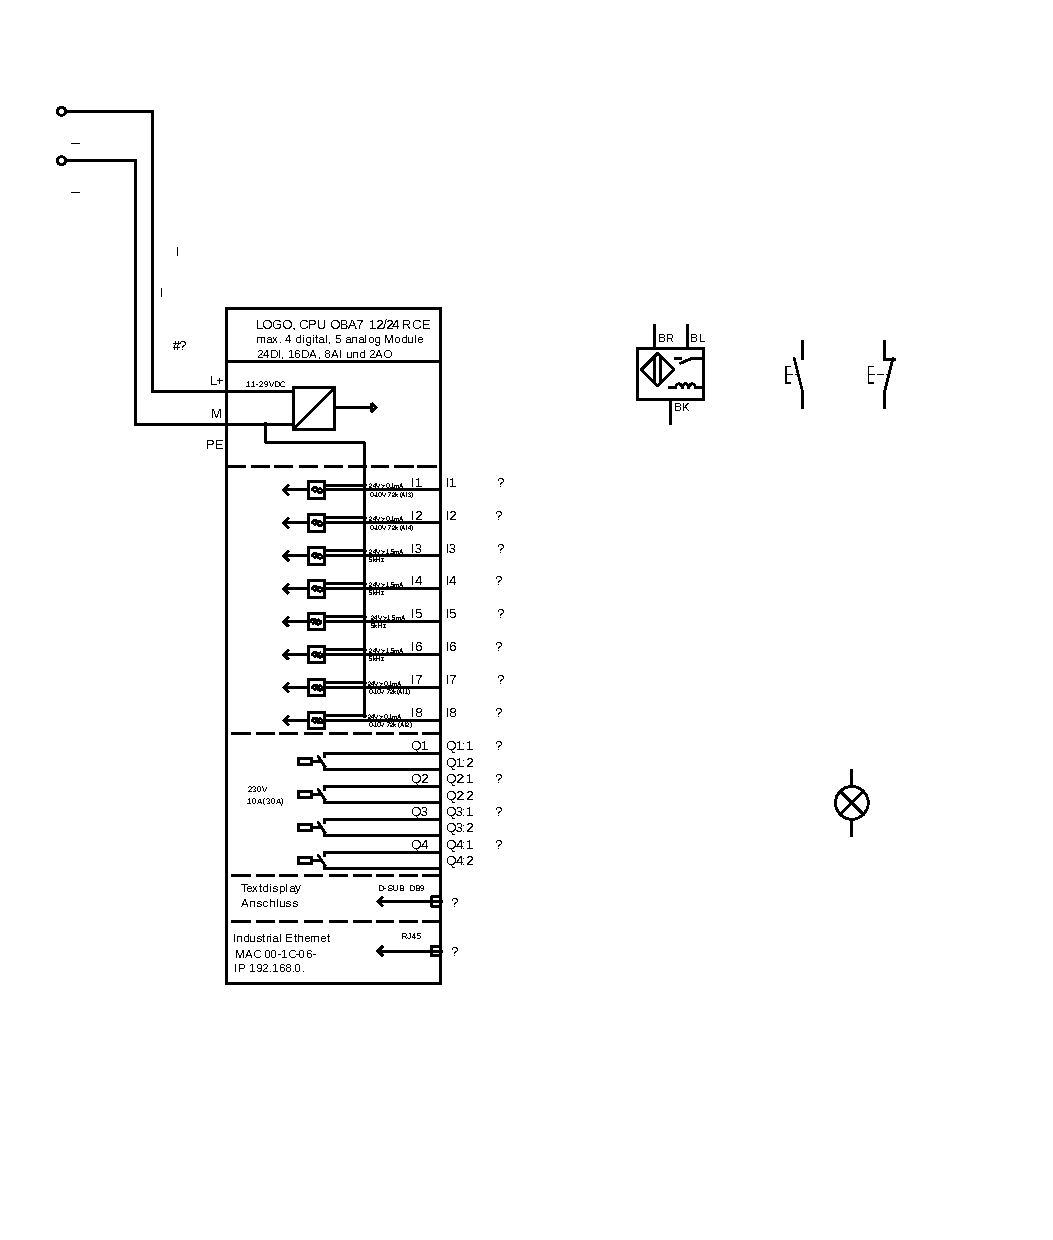
\includepdf[pages=-,pagecommand={},,, scale=0.81, trim=5mm 5mm 8mm 0, clip]{images/cablageTPtest.pdf}

}

%%%%%%%%%%%%%%%%%%%%%%%%%%%%%%%%%%%%%%%%%%%%%%%%
% Début du document
%%%%%%%%%%%%%%%%%%%%%%%%%%%%%%%%%%%%%%%%%%%%%%%%
\begin{document}
%\UPSTIobjectif{Durant cette activité, nous allons analyser une trame pour l'envoi d'informations sur une étiquette.}

%\tableofcontents
%\pagebreak


\element{combinatoire}{\section{Programme combinatoire}
	\begin{UPSTIactivite}
		\begin{question}{schemaBP}
			\checkProf[1]\\
			Sur le schéma en câblant les boutons poussoirs sur les entrées I1 et I2 de l'automate
			\vspace{-10pt}
		\end{question}

		\begin{question}{schemaVoyant}
			\checkProf[1]\\
			Compléter le schéma en câblant le voyant sur la sortie à relais Q1 de l'automate\\
			\vspace{-10pt}
		\end{question}
		%\restituegroup

		\begin{question}{cablageBP}
			\evaluationProf[2]\\
			Réaliser le cablage des boutons poussoir et du voyant en respectant un code couleur approprié
			\vspace{-10pt}
		\end{question}


		\begin{question}{voyant}
			\evaluationProf[2]\\
			Réaliser un programme qui allume le voyant lorsque le bouton poussoir rouge (Normalement fermé) n'est pas appuyé
			\vspace{-10pt}
		\end{question}

	\end{UPSTIactivite}
}
\element{sequentiel}{
	\section{Programme séquentiel}


	\UPSTIboiteCentrale{Cahier des charge séquentiel}{
		\begin{itemize}
			\item Un appui sur le bouton vert allume le voyant
			\item Le voyant reste allumé jusqu'à ce qu'un objet en métal soit détecté par le capteur inductif
		\end{itemize}
	}

	\begin{UPSTIactivite}

		\begin{question}{act2-cablageIndu}
			\checkProf[1]\\
			Compléter le schéma en câblant le capteur inductif
			\vspace{-10pt}
		\end{question}

		\begin{question}{act2-prog}
			\evaluationProf[2]\\
			Programmer le cahier des charges
			\vspace{-10pt}
		\end{question}
	\end{UPSTIactivite}
}
\element{analogique}{
\section{Entrée et sortie analogiques}

	\begin{UPSTIactivite}

		\begin{question}{act3-dessPot}
			\checkProf[1]\\
			Ajouter et dessiner le cablage d'un potentiometre sur le schéma électrique
			\vspace{-10pt}
		\end{question}


		\begin{question}{act3-cablPot}
			\checkProf[1]\\
			Câbler un potentiometre sur une entrée analogique
			\vspace{-10pt}
		\end{question}


		\begin{question}{act3-progPot}
			\evaluationProf[2]\\
			Ecrire un programme qui écrit la valeur associée au potentiometre sur l'écran du logo
			\vspace{-10pt}
		\end{question}
	\end{UPSTIactivite}
}
\element{machineAEtat}{
	\section{Machine à états}

	\UPSTIattention{Le cahier des charges de cette partie n'est pas compatible avec les programmes précédents. Après vérification des activités précédentes par un enseignant, réaliser cette partie dans un nouveau fichier}

	\UPSTIboiteCentrale{Cahier des charges}{
		\begin{enumerate}
			\item A l'appui sur le bouton poussoir, le voyant s'allume
			\item Lorsqu'une pièce métallique est détectée, le voyant clignote (utiliser le module de Asynchronious Pulse generator)
			\item Ensuite, si la tension du potentiometre vaut plus de 5V, le voyant s'éteint sur un appui sur le bouton rouge (NF)
			\item Le cycle recommence alors
		\end{enumerate}
	}

	\begin{UPSTIactivite}
		\begin{question}{act4-dessMachine}
			\evaluationProf[1]\\
			Dessiner la machine à état pour le comportement ci-dessus
			\vspace{-10pt}
		\end{question}


		\begin{question}{act4-ImpMachine}
			\evaluationProf[2]\\
			Implémenter la machine à état
			\vspace{-10pt}
		\end{question}
	\end{UPSTIactivite}
}




\csvreader[head to column names]{listeSolo.csv}{}{\sujet}

\end{document}
